\section{Задача II (навчання)}

У другому розділі розглянемо розв'язок задачі навчання: при заданій протягом часу $t=\overline{0,T}$ послiдовності спостережень $y=(y_0, \ldots , y_T)_{y_t\in F}$ слід визначити таку модель $\lambda=(\mu,A,B)$, яка максимізує ймовірність спостереження $P_\lambda(Y = y)$ вказаної послідовності $y$. Інакше кажучи, прагнемо знайти параметри моделi $\mu$, $A$ та $B$, якi найкраще пояснюють отриманi спостереження:
\begin{align*}
    \lambda^{*}=arg\max\limits_{\lambda}P_\lambda(Y=y)
\end{align*}

Означимо такі допоміжні величини:
\begin{align}
    &\gamma_t(x_t,x_{t+1})=P_\lambda(X_t=x_t,X_{t+1}=x_{t+1} \, |\, Y=y) \notag \\
    &\label{formula: gamma} \\
    &\gamma_t(x_t)=P_\lambda(X_t=x_t \, |\, Y=y)=\sum_{x_{t+1}\in E}\gamma_t(x_t,x_{t+1}) \notag
\end{align}

Величина $\gamma_t(x_t,x_{t+1})$ є ймовiрнiстю того, що в момент $t$ відбувся перехід в часі зі стану $x_t$ у стан $x_{t+1}$ при заданій послідовності спостережень $y$. А $\gamma_t(x_t)$ є сумою ймовірностей переходу від стану $x_t$ в усі можливі стани $x_{t+1}$ при відомому $y$. Зазначимо, що означені допоміжні величини можна виразити через введені у формулах \eqref{formula: alpha} й \eqref{formula: beta} ймовірності $\alpha_t(x_t)$ та $\beta_t(x_t):$
\begin{align*}
    \gamma_t(x_t,x_{t+1})&=P_\lambda(X_t=x_t,X_{t+1}=x_{t+1} \, |\, Y=y)\overset{\mathrm{def}}{=}
    \frac{P_\lambda(X_t=x_t,X_{t+1}=x_{t+1},Y=y)}{P_\lambda(Y=y)}= \\
    &=\frac{\alpha_t(x_t)\,A_{x_t x_{t+1}}B_{x_{t+1}y_{t+1}}\,\beta_{t+1}(x_{t+1})}{P_\lambda(Y=y)} \\
    \gamma_t(x_t)&=P_\lambda(X_t=x_t \, |\, Y=y)\overset{\mathrm{def}}{=}\frac{P_\lambda(X_t=x_t,Y=y)}{P_\lambda(Y=y)}=
    \frac{\alpha_t(x_t)\beta_t(x_t)}{P_\lambda(Y=y)}
\end{align*}

Ймовірність $P_\lambda(Y=y)$ легко оцінити за допомогою алгоритмів прямого чи зворотного ходу, розглянутих у попередньому розділі. 

\subsection{Алгоритм Баума-Велша}

Тож за допомогою усіх введених величин, починаючи з деякої апріорної початкової моделі $\lambda^0=(\mu^0,A^0,B^0)$, можна означити алгоритм Баума-Велша для переоцінення заданої моделі таким чином:

\begin{enumerate}
    \item Обчислюємо по формулам \eqref{formula: alpha}, \eqref{formula: beta} та \eqref{formula: gamma} 
    \begin{align*}
	    &\forall t=\overline{0,T}, \ \forall x_t \in E: && \alpha_t(x_t),\, \beta_t(x_t),\, \gamma_t(x_t) \\
        &\forall t=\overline{0,T-1}, \ \forall x_t,x_{t+1} \in E: && \gamma_t(x_t,x_{t+1})
    \end{align*}
    \item Переоцінюємо параметри моделі
    \begin{align*}
	    &\forall x_0 \in E: && \mu_{x_0}=\gamma_0(x_0) \\
        &\forall i,j \in E: && A_{ij}=\sum\limits_{t=0}^{T-1}\gamma_t(i,j) \biggl/ \ \sum\limits_{t=0}^{T-1}\gamma_t(i) \\
        &\forall i \in E, \ \forall j \in F: && B_{ij}=\sum\limits_{t=\overline{0,T},\, y_t=j}\gamma_t(i) \biggl/ \ \sum\limits_{t=0}^{T}\gamma_t(i)
    \end{align*}
    \item Обчислюємо $P_\lambda(Y=y)$ за переоціненою моделлю. Якщо ймовірність зросла менше, ніж на деяке наперед задане число $\varepsilon$, то алгоритм зупиняємо. 
\end{enumerate}

\subsection{Приклад: кмітливі учні}

За допомогою алгоритму Баума-Велша розв’яжемо задачу навчання на розглянутому у першому розділі прикладі:

\vspace{0.1cm}
\begin{mdframed}[style=text box, topline=false, bottomline=false, rightmargin=0cm, leftmargin=0cm]
    \hspace{\tabsize}
    Нехай наміри учнів незмінні: вони мають бажання відвідати футбольний матч, який відбудеться наступного тижня у середу. Проте, згідно результатів першого дослідження, учитель математики навряд чи сприятиме задуму учнів розвантажити тиждень від складного домашнього завдання. 

    Справді, математика -- складний предмет, проте не єдиний у школі. Викладачі з інших дисциплін так само задають легке, складне чи підвищеної складності домашнє завдання в залежності від піднесеного, нейтрального чи поганого настрою. Тож навіть якщо домашнє завдання з математики виявиться складним, за наявності легких завдань з решти предметів учням вдасться вправно перерозподілити час й виконати все в бажані терміни. То хто з викладачів найбільш імовірно задасть ланцюжок домашніх завдань бажаного рівня складності?
\end{mdframed}

\newpage
Нехай візьмемо за початкову модель $\lambda^0=(\mu^0,A^0,B^0)$ дані стосовно вчителя математики:

\vspace{0.4cm}
\begin{table}[H]
    \begin{minipage}[H]{0.35\linewidth}
        \begin{center}
            \begin{tabular}{c|ccc}
                & \faSmile[regular] & \faMeh[regular] & \faFrown[regular] \\
                \hline
                \faSmile[regular] & 0.2 & 0.3 & 0.5 \\
                \faMeh[regular] & 0.2 & 0.2 & 0.6 \\
                \faFrown[regular] & 0 & 0.2 & 0.8 \\
            \end{tabular}
        \end{center} \centering матриця $A^0$
    \end{minipage}
    \hfill
    \begin{minipage}[H]{0.35\linewidth}
        \begin{center}
            \begin{tabular}{c|ccc}
                & \text{\faMinus} & \text{\faRandom} & \text{\faSitemap} \\
                \hline
                \faSmile[regular] & 0.7 & 0.2 & 0.1 \\
                \faMeh[regular] & 0.3 & 0.4 & 0.3 \\
                \faFrown[regular] & 0 & 0.1 & 0.9 \\
            \end{tabular}
        \end{center} \centering матриця $B^0$
    \end{minipage}
    \hfill
    \begin{minipage}[H]{0.2\linewidth}
        \begin{center}
            \begin{tabular}{c|c}
                \faSmile[regular] & 0.05 \\
                \hline
                \faMeh[regular] & 0.2 \\
                \hline
                \faFrown[regular] & 0.75 \\
            \end{tabular}
        \end{center} \centering вектор $\mu^0$
    \end{minipage}
\end{table}

\vspace{0.4cm}
Користуючись реалізацією алгоритмів прямого та зворотного ходу (Лістинги \ref{code: alpha} та \ref{code: beta}), а також програмою обчислення коефіцієнтів $\gamma_t(x_t)$ й $\gamma_t(x_t, x_{t+1})$, наведеною нижче, проведемо процес переоцінки параметрів моделі $\lambda^0$ з метою максимізації ймовірності спостереження такої послідовності:
\begin{equation*}
    P_\lambda(Y_1=\text{\faSitemap},Y_2=\text{\faMinus},Y_3=\text{\faMinus},Y_4=\text{\faRandom},Y_5=\text{\faRandom})
\end{equation*}

Отже, програмний код матиме вид (знову ж таки, спостережені типи завдань перекодовано номерами від $1$ до $3$):

\vspace{0.4cm}
\begin{lstlisting}[firstnumber=1, label = code: gamma, caption = Обчислення коефіцієнтів $\gamma_t(i)$ та $\gamma_t(i{,}j)$]
    def gamma(y,A,B,alpha,beta,P):
        time = len(y)
        gamma_i = [[0.0 for i in range(len(B))] for t in range(time)]

        for t in range(time):
            for i in range(len(B)):
                gamma_i[t][i] = alpha[t][i]*beta[t][i]/P

        gamma_ij = [[[0.0 for j in range(len(B))] for i in range(len(B))] for t in range(time-1)]

        for t in range(time-1):
            for i in range(len(B)):
                for j in range(len(B)):
                    gamma_ij[t][i][j] = alpha[t][i]*A[i][j]*B[j][y[t+1]-1]*beta[t+1][j]/P

        return gamma_i, gamma_ij
\end{lstlisting}

\vspace{0.4cm}
Виконуватимемо ітераційний процес доти, доки ймовiрнiсть зростатиме більше, нiж на задане число $\varepsilon=0.001$. Сама функція переоцінки параметрів виглядатиме таким чином:

\newpage
\begin{lstlisting}[firstnumber=1, label = code: reestimation, caption = Переоцінення параметрів моделі]
    def reestimation(y,m,A,B,gamma_i,gamma_ij):
        time = len(y)

        for i in range(len(B)):
            m[i] = gamma_i[0][i]

        for i in range(len(B)):
            for j in range(len(B)):
                sum_i, sum_ij = 0, 0
                for t in range(time-1):
                    sum_ij += gamma_ij[t][i][j]
                    sum_i += gamma_i[t][i]
                A[i][j] = sum_ij/sum_i

        for i in range(len(B)):
            for j in range(len(B[0])):
                sum_up, sum_down = 0, 0
                for t in range(time):
                    if y[t] == j+1: sum_up += gamma_i[t][i]
                    sum_down += gamma_i[t][i]
                B[i][j] = sum_up/sum_down

        return m, A, B
\end{lstlisting}

\vspace{0.4cm}
Проміжні результати протягом $n=13$ ітерацій наведені у таблиці нижче. Відзначимо, що на перших ітераціях прирости ймовірностей зростають повільно (навіть спершу спадають), проте потім знову набирають значення. Власне, саме тому в алгоритмі Баума-Велша для зупинки навчання радять окрім встановлення порогової величини $\varepsilon$ задавати й певне число ітерацій, необхідних для виконання.

\vspace{0.4cm}
\begin{table}[H]
    \begin{center}
        \begin{tabular}{||c|S|S||}
            \hline
            Ітерація & Значення{ }ймовірності & Приріст{ }ймовірності \\
            \hline
            $k=0$ & 0.000399 & \\
            $k=1$ & 0.013765 & 0.013366 \\
            $k=2$ & 0.030787 & 0.017022 \\
            $k=3$ & 0.04689 & 0.016103 \\
            $k=4$ & 0.061967 & 0.015077 \\
            $k=5$ & 0.076644 & 0.014677 \\
            $k=6$ & 0.095408 & 0.018765 \\
            $k=7$ & 0.132333 & 0.036925 \\
            $k=8$ & 0.18631 & 0.053977 \\
            \hline
        \end{tabular}
    \end{center}
\end{table}

\begin{table}[H]
    \begin{center}
        \begin{tabular}{||c|S|S||}
            \hline
            Ітерація & Значення{ }ймовірності & Приріст{ }ймовірності \\
            \hline
            $k=9$ & 0.228093 & 0.041783 \\
            $k=10$ & 0.243223 & 0.01513 \\
            $k=11$ & 0.24704 & 0.003817 \\
            $k=12$ & 0.24818 & 0.00114 \\
            \hline
        \end{tabular}
    \end{center}
\end{table}

Отже, на момент останньої ітерації значення шуканої ймовірності дорівнює:
\begin{equation*}
    P_\lambda(Y_1=\text{\faSitemap},Y_2=\text{\faMinus},Y_3=\text{\faMinus},Y_4=\text{\faRandom},Y_5=\text{\faRandom})=0.24818
\end{equation*}

При цьому переоцінена модель $\lambda^*$ отримала такий вигляд:

\vspace{0.4cm}
\begin{table}[H]
    \begin{minipage}[H]{0.35\linewidth}
        \begin{center}
            \begin{tabular}{c|ccc}
                & \faSmile[regular] & \faMeh[regular] & \faFrown[regular] \\
                \hline
                \faSmile[regular] & 1 & 0 & 0 \\
                \faMeh[regular] & 0.53 & 0.47 & 0 \\
                \faFrown[regular] & 0 & 1 & 0 \\
            \end{tabular}
        \end{center} \centering матриця $A^*$
    \end{minipage}
    \hfill
    \begin{minipage}[H]{0.35\linewidth}
        \begin{center}
            \begin{tabular}{c|ccc}
                & \text{\faMinus} & \text{\faRandom} & \text{\faSitemap} \\
                \hline
                \faSmile[regular] & 0.05 & 0.95 & 0 \\
                \faMeh[regular] & 0.99 & 0.01 & 0 \\
                \faFrown[regular] & 0 & 0 & 1 \\
            \end{tabular}
        \end{center} \centering матриця $B^*$
    \end{minipage}
    \hfill
    \begin{minipage}[H]{0.2\linewidth}
        \begin{center}
            \begin{tabular}{c|c}
                \faSmile[regular] & 0 \\
                \hline
                \faMeh[regular] & 0 \\
                \hline
                \faFrown[regular] & 1 \\
            \end{tabular}
        \end{center} \centering вектор $\mu^*$
    \end{minipage}
\end{table}

\vspace{0.4cm}
Тож у співпраці зі старшокласниками учні можуть отримати <<математичні портрети>> усіх викладачів своєї школи, а відтак на завершальний етап дослідження школярам залишається лише співставити <<портрет>>, отриманий в результаті алгоритму навчання, із усіма наявними.

Зауважимо, що алгоритм Баума-Велша як окремий випадок EM-алгоритму є чутливим до вибору початкових параметрів, тобто моделі $\lambda^0$. Тому для чистоти експерименту учням, мабуть, не варто прив'язуватися до учителя математики, а натомість надати на вхід певний усереднений <<портрет>> викладача їхньої школи. 

Наприклад, наведемо близькі до рівномірних параметри початкової моделі $\lambda^0$ (що не обов'язково відповідає випадку конкретної школи) такого виду:

\vspace{0.4cm}
\begin{table}[H]
    \begin{minipage}[H]{0.35\linewidth}
        \begin{center}
            \begin{tabular}{c|ccc}
                & \faSmile[regular] & \faMeh[regular] & \faFrown[regular] \\
                \hline
                \faSmile[regular] & 0.4 & 0.3 & 0.3 \\
                \faMeh[regular] & 0.3 & 0.4 & 0.3 \\
                \faFrown[regular] & 0.3 & 0.3 & 0.4 \\
            \end{tabular}
        \end{center} \centering матриця $A^0$
    \end{minipage}
    \hfill
    \begin{minipage}[H]{0.35\linewidth}
        \begin{center}
            \begin{tabular}{c|ccc}
                & \text{\faMinus} & \text{\faRandom} & \text{\faSitemap} \\
                \hline
                \faSmile[regular] & 0.4 & 0.3 & 0.3 \\
                \faMeh[regular] & 0.3 & 0.4 & 0.3 \\
                \faFrown[regular] & 0.3 & 0.3 & 0.4 \\
            \end{tabular}
        \end{center} \centering матриця $B^0$
    \end{minipage}
    \hfill
    \begin{minipage}[H]{0.2\linewidth}
        \begin{center}
            \begin{tabular}{c|c}
                \faSmile[regular] & 0.3 \\
                \hline
                \faMeh[regular] & 0.4 \\
                \hline
                \faFrown[regular] & 0.3 \\
            \end{tabular}
        \end{center} \centering вектор $\mu^0$
    \end{minipage}
\end{table}

\vspace{0.4cm}
Алгоримт навчання при заданому $\varepsilon=0.001$ за таку ж кількість ітерацій $n=13$ максимізував шукану ймовірність до значення
\begin{equation*}
    P_\lambda(Y_1=\text{\faSitemap},Y_2=\text{\faMinus},Y_3=\text{\faMinus},Y_4=\text{\faRandom},Y_5=\text{\faRandom})=0.24689
\end{equation*}

При цьому модель $\lambda^*$ має вигляд:

\vspace{0.4cm}
\begin{table}[H]
    \begin{minipage}[H]{0.35\linewidth}
        \begin{center}
            \begin{tabular}{c|ccc}
                & \faSmile[regular] & \faMeh[regular] & \faFrown[regular] \\
                \hline
                \faSmile[regular] & 0.46 & 0.54 & 0 \\
                \faMeh[regular] & 0 & 1 & 0 \\
                \faFrown[regular] & 1 & 0 & 0 \\
            \end{tabular}
        \end{center} \centering матриця $A^*$
    \end{minipage}
    \hfill
    \begin{minipage}[H]{0.35\linewidth}
        \begin{center}
            \begin{tabular}{c|ccc}
                & \text{\faMinus} & \text{\faRandom} & \text{\faSitemap} \\
                \hline
                \faSmile[regular] & 0.99 & 0.01 & 0 \\
                \faMeh[regular] & 0.06 & 0.94 & 0 \\
                \faFrown[regular] & 0 & 0 & 1 \\
            \end{tabular}
        \end{center} \centering матриця $B^*$
    \end{minipage}
    \hfill
    \begin{minipage}[H]{0.2\linewidth}
        \begin{center}
            \begin{tabular}{c|c}
                \faSmile[regular] & 0 \\
                \hline
                \faMeh[regular] & 0 \\
                \hline
                \faFrown[regular] & 1 \\
            \end{tabular}
        \end{center} \centering вектор $\mu^*$
    \end{minipage}
\end{table}

\subsection{Приклад: задача кластеризації}

Розглянемо інший приклад застосування алгоритму Баума-Велша. Нехай надано великий уривок тексту (кількість символів $T\approx 50\ 000$), заданий на деякому алфавіті. Оголосимо, що кожен символ у цьому тексті слід віднести до однієї з кількох різних категорій.

Формалізуємо задачу таким чином: пара $\left\{(X_t,Y_t)\right\}_{t=\overline{0,T}}$ -- прихована марковська модель. Послідовність прихованих станів $\left\{ X_t \right\}_{t=\overline{0,T}}$ задана на множині категорій $E=\left\{e_1,e_2, \ldots, e_N\right\}$, а послідовність спостережуваних символів $\left\{ Y_t \right\}_{t=\overline{0,T}}$ задана на алфавіті $F=\left\{f_1,f_2, \ldots, f_M\right\}$ деякої мови.

Суть задачі кластеризації літер зводитиметься до аналізу переоціненої в результаті алгоритму Баума-Велша певної початкової моделі $\lambda^0=(\mu^0,A^0,B^0)$, сформованої за припущеннями про наданий текст. Проте, перш ніж рухатися безпосередньо до кластеризації, слід врахувати деякі зміни в роботі самого алгоритму. Розглянемо ці зміни у двох наступних підрозділах: <<Шкалювання алгоритмів прямого та зворотного ходу>> й <<Критерій зупинки алгоритму>>.

\subsubsection{Шкалювання алгоритмів прямого та зворотного ходу}

Перш за все, через значну довжину вектора спостережуваних станів (тобто в силу того, що текст складається з великої кількості символів), значення коефіцієнтів $\alpha_t(x_t)$ і $\beta_t(x_t)$ з кожною наступною ітерацією будуть стрімко прямувати до нуля, що можна помітити у таблицях проміжних результатів алгоритмів прямого та зворотного ходу (сторінка \pageref{table: forward/backward algorithms}).

Відтак не кожна програма буде в змозі оперувати з величинами такої мализни. Одним з рiшень цiєї проблеми є процедура шкалювання (ще кажуть нормування) відповідних ймовірностей.

Отже, одразу після обчислення на черговому кроці $t$ коефіцієнтів за формулами \eqref{formula: alpha} та \eqref{formula: beta} додають крок переоцінки:
\begin{equation*}
    \widehat{\alpha}_t(i) = \frac{\alpha_t(i)}{\sum\limits_{j \in E}\alpha_t(j)}, \ 
    \widehat{\beta}_t(i) = \frac{\beta_t(i)}{\sum\limits_{j \in E}\beta_t(j)} 
\end{equation*}

А тоді коефіцієнти \eqref{formula: gamma} слід обчислювати наступним чином:
\begin{equation*}
    \gamma_t(i)= \frac{\widehat{\alpha}_t(i)\,\widehat{\beta}_t(i)}{\sum\limits_{j \in E}\widehat{\alpha}_t(j)\,\widehat{\beta}_t(j)}, \
    \gamma_t(i,j)=\frac{\widehat{\alpha}_t(i)\,A_{ij}\,B_{jy_{t+1}}\,\widehat{\beta}_{t+1}(j)}
        {\sum\limits_{k \in E}\sum\limits_{w \in E}\widehat{\alpha}_t(k)\,A_{kw}\,B_{wy_{t+1}}\,\widehat{\beta}_{t+1}(w)}
\end{equation*}

Процедура нормування має декілька різних модифікацій. Наприклад\catcode`\%=12 \footnote{
    Mikael Nilsson, \href{https://www.google.com/url?sa=t&rct=j&q=&esrc=s&source=web&cd=&cad=rja&uact=8&ved=2ahUKEwjYpp2ix577AhWgi_0HHWj2CgIQFnoECAwQAQ&url=https%3A%2F%2Fwww.semanticscholar.org%2Fpaper%2FFirst-Order-Hidden-Markov-Model-%253A-Theory-and-Issues-Nilsson%2Fb377061fca96921bc12dcc3609ddc9e526d96daf&usg=AOvVaw0-xnjeeFXADozjvvUFlOPQ}
    {<<First Order Hidden Markov Model: Theory and Implementation Issues>>}}, 
в одному з варіантів на кроці $t$ коефіцієнти спершу алгоритму прямого, а за ними й коефіцієнти алгоритму зворотного ходу шкалюють однаковими нормуючими множниками такого виду:
\begin{equation}
    c_t = \frac{1}{\sum\limits_{j \in E}\alpha_t(j)}
    \label{formula: scaling coefficients}
\end{equation}

Водночас, інші дослідження\catcode`\%=12 \footnote{
    Mark Hasegawa-Johnson, \href{https://www.google.com/url?sa=t&rct=j&q=&esrc=s&source=web&cd=&ved=2ahUKEwiL1Y-rt577AhXdxQIHHReZCksQFnoECAsQAQ&url=https%3A%2F%2Fcourses.engr.illinois.edu%2Fece417%2Ffa2020%2Fslides%2Flec14.pdf&usg=AOvVaw0Y9Q3DuoKI0YP8XBedlu_H}
    {<<Lecture 14: Log Viterbi and Scaled Forward-Backward>>}}
стверджують, що такі зміни не внесуть значної переваги. Зокрема, у ході власних спостережень також не вдалося помітити значущої відмінності отриманих результатів чи різниці швидкості збіжності алгоритму в залежності від способу нормування.  

\subsubsection{Критерій зупинки алгоритму}

Стосовно критерію зупинки алгоримту навчання, то, враховуючи модифікації коефіцієнтів $\alpha_t(x_t)$ та $\beta_t(x_t)$, замість відстеження від ітерації до ітерації безпосередніх приростів імовірностей спостереження бажаної послідовності, слід обчислювати зміну відповідних логарифмів імовірностей, побудованих через коефіцієнти нормування \eqref{formula: scaling coefficients} таким чином:
\begin{equation}
    \ln P(Y=y) = -\sum\limits_{t=0}^{T}\ln c_t
    \label{formula: stop criterion}
\end{equation}

Отже, процес переоцінки параметрів моделі можна припиняти тоді, коли приріст логарифмів імовірностей припиняє перевищувати деяке наперед задане число $\varepsilon$.

В межах задачі поділу літер деякого алфавіту на кілька різних категорій, визначимо оптимальне порогове значення $\varepsilon$ через дослідження збіжності результатів самої кластеризації. Інакше кажучи, необхідно знайти величину приросту $\Delta\ln P(Y=y)$, за якої модель досягає такого стану, що результати задачі кластеризації перестають істотно змінюватися. 

Побудуємо аналіз збіжності результатів задачі кластеризації таким чином: замість введення міри схожості результатів двох послідовних ітерацій, введемо функцію подібності для поточного результату та деякого еталонного виходу, отриманого заздалегідь протягом роботи дуже великої кількості ітерацій $(n=200,400,600)$. Доречність вибору такого способу відстеження збіжності буде наочно продемонстрована у наступних підрозділах.   

Тож нехай результати поточного групування літер на деякій ітерації $n$ позначимо як $\mathbf{G^n}=(\mathbf{G}_i^n)_{i\in E}$, а еталонні групи -- як $\mathbf{G^*}=(\mathbf{G}_i^*)_{i\in E}$. Тоді функцію подібності $\delta$ між результатами $\mathbf{G^n}$ та $\mathbf{G}^*$ покладемо так:
\begin{equation}
    \delta(\mathbf{G^n}, \mathbf{G}^*)=\frac{1}{|E|}\cdot\sum\limits_{i\in E}\frac{\sum\limits_{j\in \mathbf{G}_i^n}\mathds{1}(j\in\mathbf{G}_i^*)}{\max\bigl\{ |\mathbf{G}_i^n|,|\mathbf{G}_i^*| \bigr\}}
    \label{formula: measure of similarity}
\end{equation}

Фактично, міра \eqref{formula: measure of similarity} є середнім арифметичним між відношеннями попарного порівняння відповідних поточних та еталонних груп, тобто відсотковими співвідношеннями виду:
\vspace{0.2cm}
\begin{equation*}
    \frac{\text{кількість збігів поточного класу з еталонним}}
    {\text{загальна кількість літер або у поточному класі, або в еталонному}}
\end{equation*}

\vspace{0.2cm}
Розглянемо специфіку роботи введеної міри на такому прикладі: нехай в результаті $n=400$ ітерацій алгоритму навчання деякої початкової моделі отримано такий розподіл літер англійського алфавіту на три кластери:
\begin{align*}
    & \text{група } \mathbf{G}_\text{I}^* && \parbox{12cm}{<<a>>, <<e>>, <<i>>, <<o>>, <<q>>, <<u>>} \\
    & \text{група } \mathbf{G}_\text{IІ}^* && \parbox{12cm}{<<c>>, <<d>>, <<f>>, <<k>>, <<l>>, <<m>>, <<n>>, <<r>>, <<s>>, <<v>>, <<x>>, <<z>>} \\
    & \text{група } \mathbf{G}_\text{IІI}^* && \parbox{12cm}{<<b>>, <<g>>, <<h>>, <<j>>, <<p>>, <<t>>, <<w>>, <<y>>}
\end{align*}

Вважатимемо ці результати еталонними. Натомість, під час іншого запуску алгоритму Баума-Велша для такої ж початкової моделі на $n=50$ ітерації отримано розподіл такого виду:
\begin{align*}
    & \text{група } \mathbf{G}_\text{I}^{\text{\scriptsize 50}} && \parbox{12cm}{<<a>>, <<e>>, <<i>>, <<o>>, <<q>>, <<u>>, <<x>>, <<z>>} \\
    & \text{група } \mathbf{G}_\text{IІ}^{\text{\scriptsize 50}} && \parbox{12cm}{<<c>>, <<d>>, <<f>>, <<k>>, <<l>>, <<m>>, <<n>>} \\
    & \text{група } \mathbf{G}_\text{IІI}^{\text{\scriptsize 50}} && \parbox{12cm}{<<b>>, <<g>>, <<h>>, <<j>>, <<p>>, <<t>>, <<w>>, <<y>>, <<r>>, <<s>>, <<v>>}
\end{align*}

Обчислимо відношення подібності між парою груп $\mathbf{G}_\text{I}^{\text{\scriptsize 50}}$ та $\mathbf{G}_\text{I}^*:$ кількість збігів між цими класами рівна $6$, в той час як загальна кількість символів у групі $\mathbf{G}_\text{I}^{\text{\scriptsize 50}}$ рівна~$8$. Отже, схожіть цих груп оцінюватиметься у $75\%$. Аналогічним чином обчислимо подібність між категоріями $\mathbf{G}_\text{IІ}^{\text{\scriptsize 50}}$ та $\mathbf{G}_\text{IІ}^*:$ кількість збігів рівна $7$, а кількість символів в еталонному класі $\mathbf{G}_\text{IІ}^*$ -- $12$. Відповідно, відсоток схожості дорівнює $58\%$. Для останної пари кластерів відсоток подібності рівний $73\%$. Отже, міра схожості $\delta$ для груп $\mathbf{G^{\text{\scriptsize 50}}}$ та $\mathbf{G}^*$ записуватиметься так:
\begin{equation*}
    \delta(\mathbf{G^{\text{\scriptsize 50}}}, \mathbf{G}^*)=\frac{1}{3}(75\% + 58\% + 73\%) = 69\%
\end{equation*}

\newpage
Отже, зважаючи на збіжні властивості алгоритму Баума-Велша, рано чи пізно міра схожості \eqref{formula: measure of similarity} зросте аж до стовідсоткового значення. Тож фіксуючи протягом роботи алгоритму прирости $\Delta\ln P(Y=y)$ та відповідні показники міри подібності, є можливість відстежити оптимальне значення порогової величини $\varepsilon$, за якого алгоритм навчання можна припиняти. В ключі швидкодії алгоритму, такі спостереження будуть цінними Конкретні приклади та висновки стосовно значення $\varepsilon$ будуть розглянуті для кожної задачі кластеризації окремо.

\subsubsection{Підготовчий етап}

Озброївшись введеними модифікаціями й уточненнями алгоритму Баума-Велша, кластеризуймо літери українського алфавіту, розглянувши текст перших трьох глав роману <<Місто>> україномовного автора Валер'яна Підмогильного. 

Проте, перш за все виконаємо підготовчий етап, залишивши в тексті лише букви одного регістру, знаки пробілу та апострофа. Наприклад, оглянемо такий уривок:

\vspace{0.3cm}
\begin{mdframed}[style=text box]
    \hspace{\tabsize}\textsl{
    На вулиці йому спала раптова думка. Що коли зайти в яку велику установу? Може, там якраз випадково, потрібен молодий кмітливий рахівник чи реєстратор? Просто зайти й спитати. Це ж не гріх. Скажуть немає, то й піде. А раптом пощастить? Ця думка схвилювала його. В душі йому жила міцна надія на свою долю, бо кожному властиво вважати себе за цілком виключне явище під сонцем і місяцем. Він звернув до ґанку під великою вивіскою <<Державне видавництво України>> і швидким кроком зійшов на другий поверх.}
\end{mdframed}

\vspace{0.3cm}
Цей же уривок тексту після <<чистки>>:

\vspace{0.3cm}
\begin{mdframed}[style=text box]
    \hspace{\tabsize}\textsl{
    на вулиці йому спала раптова думка що коли зайти в яку велику установу може там якраз випадково потрібен молодий кмітливий рахівник чи реєстратор просто зайти й спитати це ж не гріх скажуть немає то й піде а раптом пощастить ця думка схвилювала його в душі йому жила міцна надія на свою долю бо кожному властиво вважати себе за цілком виключне явище під сонцем і місяцем він звернув до ґанку під великою вивіскою державне видавництво україни і швидким кроком зійшов на другий поверх}
\end{mdframed}

\vspace{0.3cm}
Такого роду редагування можна виконати або за допомогою вбудованих функцій різних текстових редакторів, або самостійно написавши невеликий скрипт аналогічного призначення на обраній мові програмування. 

Отже, на кінець підготовчого етапу отримуємо текст ($T=45\; 070$ символів), заданий на алфавіті $F$ довжиною $M=35$ елементи ($33$ літери, пробіл та апостроф):
\begin{equation}
    F=\{\text{<<а>>},\text{<<б>>},\text{<<в>>},\ldots,\text{<<ь>>},\text{<<ю>>},\text{<<я>>},\text{<< >>},\text{<<'>>}\}
    \label{formula: UKR alphabet}
\end{equation}

\newpage
\subsubsection{Кластеризація літер на дві категорії}
\label{section: II classes}

Розглянемо приховану марковську модель на декартовому добутку $E\times F$, де $E=\left\{\text{I},\text{II}\right\}$ -- множина двох категорій, а $F$ є алфавітом, отриманим після підготовчого етапу. Нехай про особливості самого алфавіту нам нічого не відомо, а тому початкову модель $\lambda^0=(\mu^0,A^0,B^0)$ покладемо близькою до рівномірної:

\vspace{0.4cm}
\begin{table}[H]
    \begin{minipage}[H]{0.35\linewidth}
        \begin{center}
            \begin{tabular}{c|ccc}
                & I & II \\
                \hline
                I & 0.4 & 0.6 \\
                II & 0.6 & 0.4 \\
            \end{tabular}
        \end{center} \centering матриця $A^0$
    \end{minipage}
    \hfill
    \begin{minipage}[H]{0.35\linewidth}
        \begin{center}
            \begin{tabular}{c|ccc}
                & $f_1$ & $\ldots$ & $f_M$ \\
                \hline
                I & $\sim \frac{1}{M}$ & $\ldots$ & $\sim \frac{1}{M}$ \\
                II & $\sim \frac{1}{M}$ & $\ldots$ & $\sim \frac{1}{M}$ \\
            \end{tabular}
        \end{center} \centering матриця $B^0$
    \end{minipage}
    \hfill
    \begin{minipage}[H]{0.25\linewidth}
        \begin{center}
            \begin{tabular}{c|c}
                I & 0.4 \\
                \hline
                II & 0.6 \\
            \end{tabular}
        \end{center} \centering вектор $\mu^0$
    \end{minipage}
\end{table}

\vspace{0.4cm}
Один із варіантів програмної реалізації заповнення елементів початкової матриці $B^0$ рівномірними, але водночас неоднаковими, значеннями полягає у фомуванні комірок в два кроки: спершу заповнимо елементи матриці  згідно такого правила:
\begin{equation*}
    \widetilde{B}_{ij}=\tfrac{1}{M} + \xi_{ij}, \text{ де } \xi_{ij}\sim U(-0.01,\, 0.01), 
\end{equation*}

де випадкова величина $\xi$ має рівномірний розподіл на відрізку, при цьому математичне сподівання $\xi$ дорівнює нулю, а дисперсія є малою. А тоді задля виконання умови стохастичності, наступним кроком зробимо нормування по рядкам $i\in E$:
\begin{equation*}
    B_{ij}^0=\frac{\widetilde{B}_{ij}}{\sum\limits_{j=1}^{M}\widetilde{B}_{ij}}
\end{equation*}

\subsubsection*{Результати}

Проаналізуємо модель $\lambda^*=(A^*,B^*,\mu^*)$, отриману в результаті $n=400$ ітерацій алгоритму Баума-Велша. Вiднесемо кожен символ алфавіту $F$ до одного з двох класiв І або ІІ, порiвнявши для кожного елемента $j\in F$ ймовiрностi $B_{\text{I}j}^*$ та $B_{\text{II}j}^*:$
\begin{equation}
    \begin{aligned}
        & \text{I категорія} && \parbox{12cm}{<<а>>, <<е>>, <<и>>, <<о>>, <<у>>, <<ь>>, <<я>>, <<і>>} \\
        & \text{II категорія} && \parbox{12cm}{\vspace{0.2cm} <<б>>, <<в>>, <<г>>, <<д>>, <<ж>>, <<з>>, <<й>>, <<к>>, <<л>>, <<м>>, <<н>>, <<п>>, <<р>>, <<с>>, <<т>>, <<ф>>, <<х>>, <<ц>>, <<ч>>, <<ш>>, <<щ>>, <<ґ>>, <<ї>>, <<є>>, <<ю>>, << >>, <<'>>}
    \end{aligned}
    \label{formula: II classes}
\end{equation}

За вийнятком окремих символів, літери з першої категорії позначають на письмі голосні звуки українського алфавіту, а літери з другої категорії -- приголосні. Віднесення букв <<ї>>, <<є>> та <<ю>> до групи II можна пояснити тим, що кожен такий символ складається з двох частин, перша з яких -- приголосний звук <<й>>.

Переоцінена матриця $A^*$, в свою чергу, містить інформацію щодо ймовірностей переходів між класами I та II. Відтак, перехід з голосної літери у приголосну (тобто компонента $A_{\text{I,II}}^*$) має найбільшу ймовірність, а перехід $A_{\text{I,I}}^*$ з голосної у голосну -- найменшу. Такі результати цілком узгоджуються з особливостями чергування голосних та приголосних в українській мові:

\vspace{0.4cm}
\begin{table}[H]
    \begin{center}
        \begin{tabular}{c|ccc}
            & I & II \\
            \hline
            I & 0.01 & 0.99 \\
            II & 0.64 & 0.36 \\
        \end{tabular}
    \end{center} \centering матриця $A^*$
\end{table}

\vspace{0.4cm}
Підійдемо до спроб охарактеризувати збіжні властивості алгоритму кластеризації літер на дві категорії. Користуючись мірою подібності \eqref{formula: measure of similarity}, відстежимо від ітерації до ітерації схожість результатів з еталонним виходом \eqref{formula: II classes}:
\subfiguresbegin
\begin{figure}[H]
    \center{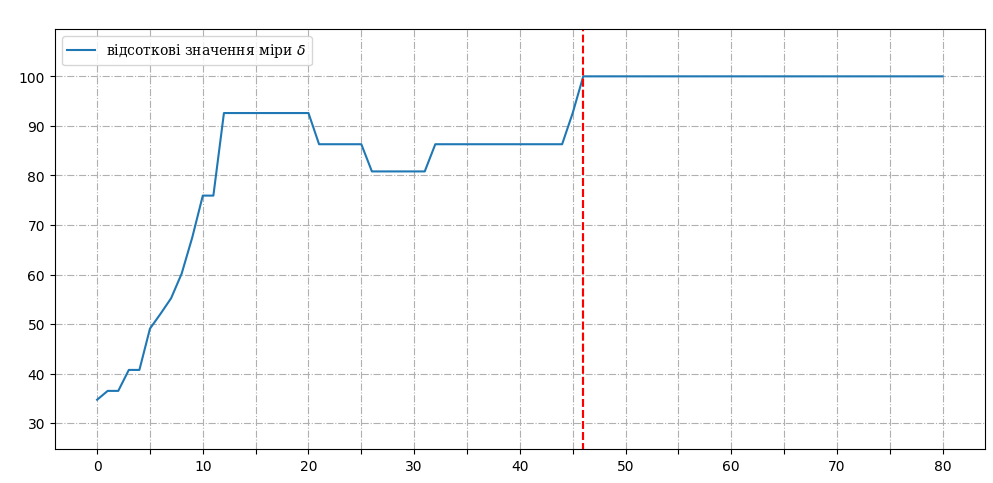
\includegraphics[width=1\linewidth]{2D_delta.png}}
    \vspace{-0.5cm}
    \caption{\label{first} Значення $\delta$ (вісь ординат) від ітерації до ітерації (вісь абсцис)}
    \label{figure: II delta}
\end{figure}

Червоною вертикальною прямою позначена перша ітерація, коли результат збігається з еталоном. Таким чином, вже на $n=46$ ітерації поділ літер на голосні-приголосні набуває остаточного, фінального вигляду. 

Водночас, з графіку видно, що протягом значного часу (наприклад, від ітерації $n=32$ до $n=44$) розподіл літер лишається незмінним, але все ще недосконалим ($\approx 86\%$ схожості). Саме тому побудова міри подібності \eqref{formula: measure of similarity} ґрунтувалася на схожості поточних результатів з еталонними на противагу порівнянню сусідніх результатів кластеризації. 

Фіксуючи з кожною ітерацією значення приростів $\varepsilon=\Delta\ln P(Y=y)$, отримуємо такі спостереження:
\begin{figure}[H]
    \center{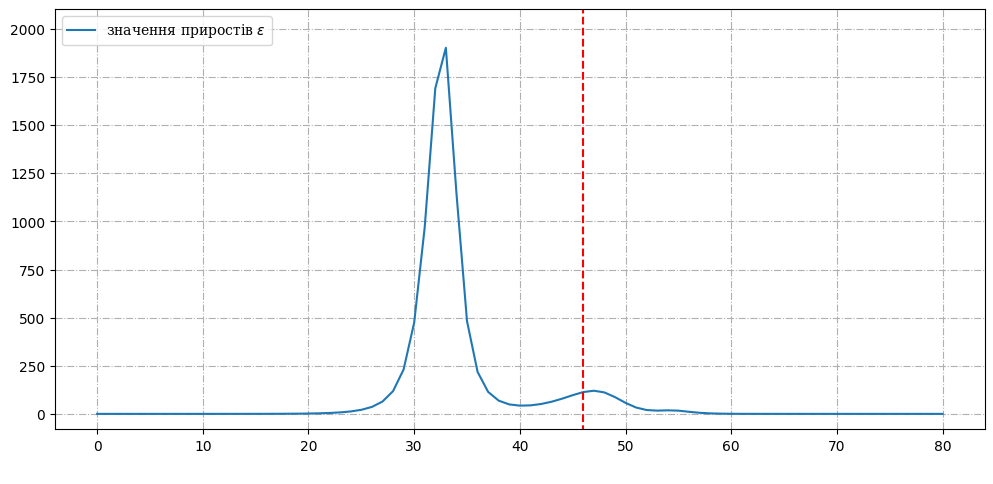
\includegraphics[width=1\linewidth]{2D_epsilon.png}}
    \vspace{-0.8cm}
    \caption{\label{second} Значення $\varepsilon$ (вісь ординат) від ітерації до ітерації (вісь абсцис)}
    \label{figure: II epsilon}
\end{figure}
\subfiguresend

Бачимо, що зростання починає відбуватися не одразу, алгоритму необхідний деякий час, аби <<розігнатися>>. Саме про цей ефект йшла мова при розв'язанні прикладу кмітливих учнів (сторінка \pageref{code: reestimation}). Крім того, цікавим є факт, що перший збіг з еталоном припадає не на ітерації найбільшого зростання. 

Оминувши інформацію про надвеликі значення приростів $\varepsilon$, розглянемо графік більш детально:
\begin{figure}[H]
    \center{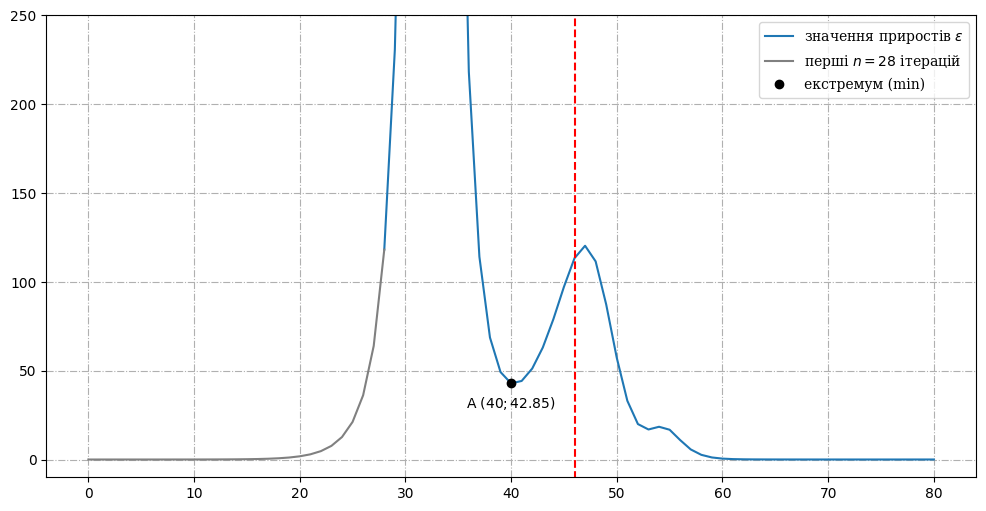
\includegraphics[width=1\linewidth]{2D_epsilon_zoom.png}}
    \vspace{-0.8cm}
    \caption{Значення $\varepsilon$ на проміжку $(0,250)$}
    \label{figure: II epsilon (0,250)}
\end{figure}

\newpage
Проаналізувавши наведений графік, виявимо оптимальний критерій зупинки алгоритму Баума-Велша для випадку кластеризації на дві категорії. Тож нехай перші $n=28$ ітерацій є обов'язковими до виконання (позначимо ці <<ітерації для розгону>> сірим кольором). 

Тоді, фактично, оптимальною пороговою величиною $\varepsilon^*$ є значення найменшого серед усіх екстремумів (а саме: мінімумів), наявних до ітерації першого збігу з еталоном. У даному випадку єдиним таким мінімумом є точка $A$ з координатами $(40, 42.85)$, тобто на ітерації $n=40$ зі значенням приросту $\varepsilon=42.85$ (ця точка позначена чорною крапкою). 

Отже, виконавши декілька десятків обов'язкових ітерацій, алгоримт навчання може зупинятися тоді, коли вперше спорігатиме приріст $\varepsilon^*<42.85$. 

\subsubsection{Кластеризація літер на три категорії}
\label{section: III classes}

Продемонструємо результати поділу літер на більш ніж два класи: введемо приховану марковську модель на множині трьох категорій $E=\left\{\text{I},\, \text{II},\, \text{IIІ}\right\}$ та на отриманому раніше алфавіті \eqref{formula: UKR alphabet}:
\begin{equation*}
    F=\{\text{<<а>>},\text{<<б>>},\text{<<в>>},\ldots,\text{<<ь>>},\text{<<ю>>},\text{<<я>>},\text{<< >>},\text{<<'>>}\}
\end{equation*}

Початкову модель $\lambda^0=(\mu^0,A^0,B^0)$ знову покладемо близькою до рівномірної:

\vspace{0.4cm}
\begin{table}[H]
    \begin{minipage}[H]{0.35\linewidth}
        \begin{center}
            \begin{tabular}{c|cccc}
                & I & II & III \\
                \hline
                I & 0.4 & 0.3 & 0.3 \\
                II & 0.3 & 0.4 & 0.3 \\
                III & 0.3 & 0.3 & 0.4 \\
            \end{tabular}
        \end{center} \centering матриця $A^0$
    \end{minipage}
    \hfill
    \begin{minipage}[H]{0.4\linewidth}
        \begin{center}
            \begin{tabular}{c|ccc}
                & $f_1$ & $\ldots$ & $f_{35}$ \\
                \hline
                I & $\sim \frac{1}{35}$ & $\ldots$ & $\sim \frac{1}{35}$ \\
                II & $\sim \frac{1}{35}$ & $\ldots$ & $\sim \frac{1}{35}$ \\
                III & $\sim \frac{1}{35}$ & $\ldots$ & $\sim \frac{1}{35}$ \\
            \end{tabular}
        \end{center} \centering матриця $B^0$
    \end{minipage}
    \hfill
    \begin{minipage}[H]{0.2\linewidth}
        \begin{center}
            \begin{tabular}{c|c}
                I & 0.3 \\
                \hline
                II & 0.4 \\
                \hline
                III & 0.3 \\
            \end{tabular}
        \end{center} \centering вектор $\mu^0$
    \end{minipage}
\end{table}

\vspace{0.4cm}
Проаналiзуваши матрицю $B^*$, отриману після $n=400$ iтерацiй алгоритму Баума-Велша, отримуємо результати:
\begin{equation}
    \begin{aligned}
        & \text{I категорія} && \parbox{10cm}{<<б>>, <<в>>, <<г>>, <<д>>, <<ж>>, <<к>>, <<л>>, <<м>>, <<н>>, <<п>>, <<р>>, <<т>>, <<ф>>, <<ц>>, <<ч>>, <<ш>>, <<щ>>, <<ґ>> \vspace{0.1cm}} \\
        & \text{II категорія} && \parbox{10cm}{<<а>>, <<е>>, <<и>>, <<о>>, <<у>>, <<ь>>, <<я>>, <<і>>, << >>} \\
        & \text{III категорія} &&  \parbox{10cm}{<<з>>, <<й>>, <<с>>, <<х>>, <<ї>>, <<є>>, <<ю>>, <<’>>}
    \end{aligned}
    \label{formula: III classes}
\end{equation}

Бачимо, що категорію І складають літери на позначення приголосних звуків, а категорію ІІ -- на позначення голосних. Категорія ІІІ містить приголосний <<й>>, парні по дзвінкості букви <<з>> та <<с>>, глухий <<x>> та букви <<ї>>, <<є>>, <<ю>>, які самі по собі складаються з двох звуків, один з яких -- <<й>>.

Аналогічним до попереднього розділу чином зобразимо спостереження стосовно збіжності алгоритму кластеризації на три категорії:

\begin{figure}[H]
    \begin{minipage}[H]{1\linewidth}
        \center{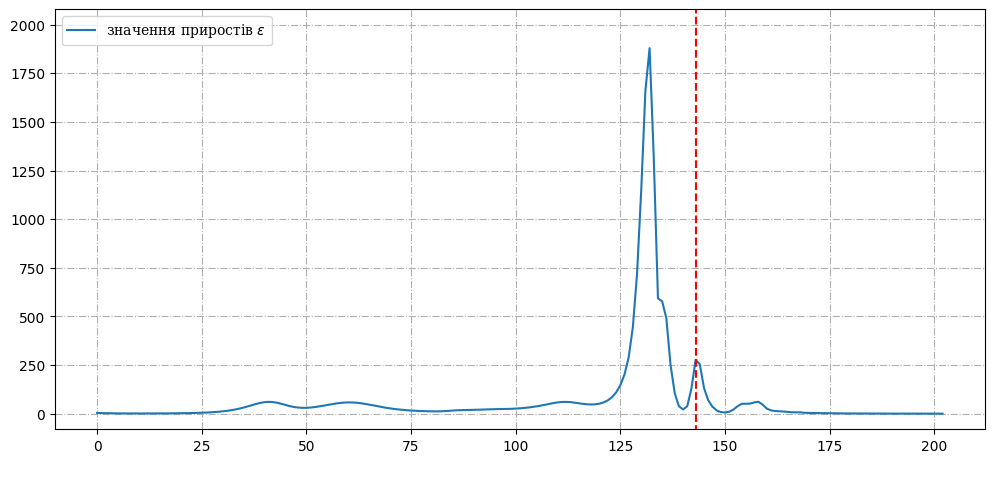
\includegraphics[width=1\linewidth]{3D_epsilon.png}}
    \end{minipage}
    \vspace{0.5cm}
    \begin{minipage}[H]{1\linewidth}
        \center{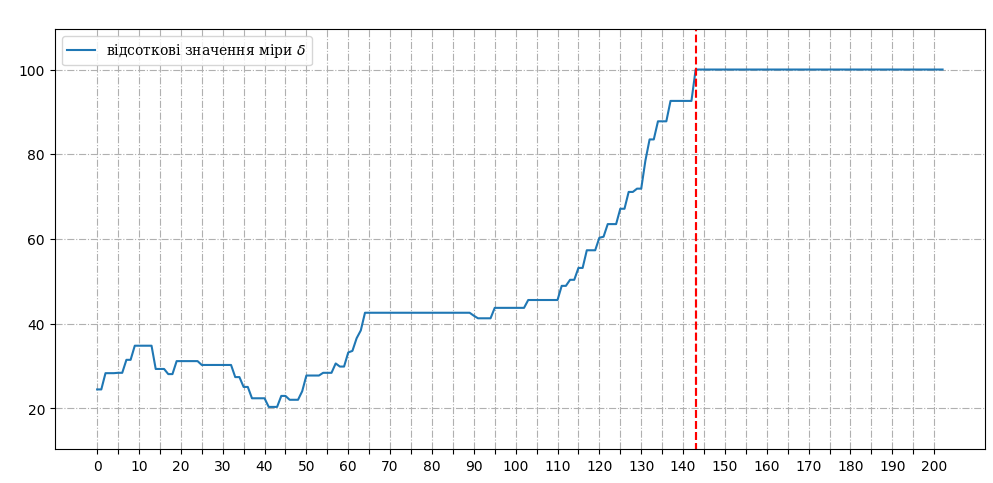
\includegraphics[width=1\linewidth]{3D_delta.png}}
    \end{minipage}
    \vspace{-0.4cm}
    \caption{Значення приростів $\varepsilon$ та міри $\delta$ від ітерації до ітерації}
    \label{figure: III epsilon & delta}
\end{figure}

Отже, вже на ітерації $n=143$ результати задачі кластеризації збігаються з еталоном \eqref{formula: III classes}, причому перший збіг знову потрапляє не в множину ітерацій найбільного <<піку>> зростання різниць $\Delta\ln P(Y=y)$. Розглянемо детальніше графік приростів $\varepsilon$ (Рис. \ref{figure: III epsilon (0,90)}), аби віднайти оптимальне порогове значення зупинки алгоритму навчання.

Нехай перші $n=35$ ітерацій алгоритму покладемо обов'язковими до виконання (позначимо їх сірим кольором). Тоді значення $\varepsilon^*$ буде визначатися як найменше число $\varepsilon$ серед точок мінімумів, наявних до ітерації першого збігу з фінальним результатом, тобто серед точок $A,B,C,D$ або $E$, позначених чорними крапками.

\begin{figure}[H]
    \center{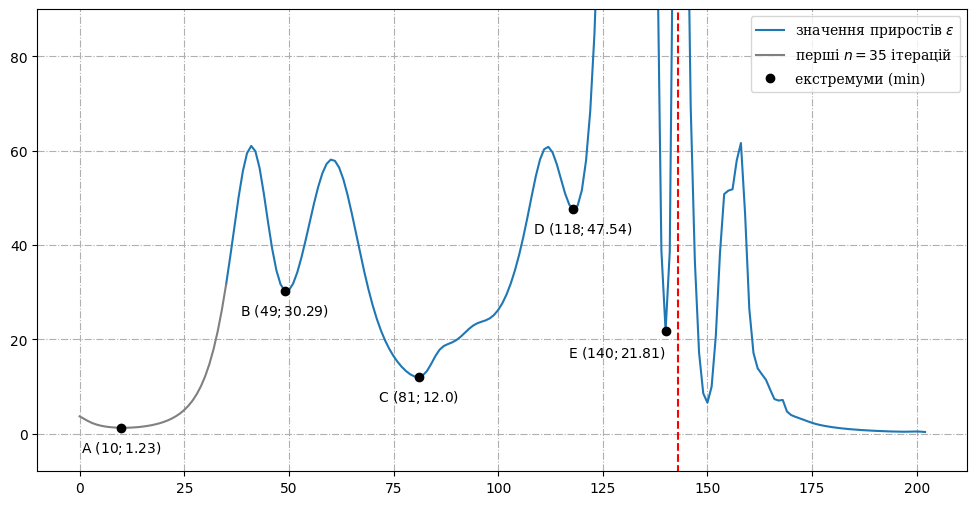
\includegraphics[width=1\linewidth]{3D_epsilon_zoom.png}}
    \vspace{-0.7cm}
    \caption{Значення $\varepsilon$ на проміжку $(0,90)$}
    \label{figure: III epsilon (0,90)}
\end{figure}

Однак, точка $A$ входить у сіру область перших $n=35$ ітерацій, а відтак, цю точку можна викреслити з множини претендентів на оптимальну порогову величину. Отже, серед множини точок, які лишилися, точка $C$ має наменшу координату, а тому робимо висновок, що, виконавши декiлька десяткiв обов’язкових iтерацiй, алгоримт навчання можна зупиняти при першому спостереженні приросту $\varepsilon^*<12$.

\subsubsection{Кластеризація літер на чотири категорії}
\label{section: IV classes}

Нарешті, поділимо літери на чотири групи: розглянемо приховану марковську модель на множині чотирьох категорій $E=\left\{\text{I},\, \text{II},\, \text{IIІ},\, \text{IV}\right\}$ та алфавіті \eqref{formula: UKR alphabet}:
\begin{equation*}
    F=\{\text{<<а>>},\text{<<б>>},\text{<<в>>},\ldots,\text{<<ь>>},\text{<<ю>>},\text{<<я>>},\text{<< >>},\text{<<'>>}\}
\end{equation*}

Початкову модель $\lambda^0=(\mu^0,A^0,B^0)$ покладемо близькою до рівномірної:

\vspace{0.4cm}
\begin{table}[H]
    \begin{minipage}[H]{0.4\linewidth}
        \begin{center}
            \begin{tabular}{c|ccccc}
                & I & II & III & IV \\
                \hline
                I & 0.3 & 0.2 & 0.2 & 0.3 \\
                II & 0.2 & 0.3 & 0.3 & 0.2 \\
                III & 0.3 & 0.2 & 0.2 & 0.3 \\
                IV & 0.2 & 0.3 & 0.3 & 0.2 \\
            \end{tabular}
        \end{center} \centering матриця $A^0$
    \end{minipage}
    \hfill
    \begin{minipage}[H]{0.38\linewidth}
        \begin{center}
            \begin{tabular}{c|ccc}
                & $f_1$ & $\ldots$ & $f_{35}$ \\
                \hline
                I & $\sim \frac{1}{35}$ & $\ldots$ & $\sim \frac{1}{35}$ \\
                II & $\sim \frac{1}{35}$ & $\ldots$ & $\sim \frac{1}{35}$ \\
                III & $\sim \frac{1}{35}$ & $\ldots$ & $\sim \frac{1}{35}$ \\
                IV & $\sim \frac{1}{35}$ & $\ldots$ & $\sim \frac{1}{35}$ \\
            \end{tabular}
        \end{center} \centering матриця $B^0$
    \end{minipage}
    \hfill
    \begin{minipage}[H]{0.16\linewidth}
        \begin{center}
            \begin{tabular}{c|c}
                I & 0.2 \\
                \hline
                II & 0.3 \\
                \hline
                III & 0.2 \\
                \hline
                IV & 0.3 \\
            \end{tabular}
        \end{center} \centering вектор $\mu^0$
    \end{minipage}
\end{table}

\vspace{0.4cm}
В результаті $n=400$ iтерацiй маємо такий розподіл:
\begin{equation}
    \begin{aligned}
    & \text{I категорія} && \parbox{10cm}{<<л>>, <<н>>, <<р>>, <<ц>>, <<’>>} \\
    & \text{II категорія} && \parbox{10cm}{<<з>>, <<й>>, <<с>>, <<ї>>, <<є>>, <<ю>>, << >>} \\
    & \text{III категорія} &&  \parbox{10cm}{<<б>>, <<в>>, <<г>>, <<д>>, <<ж>>, <<к>>, <<м>>, <<п>>, <<т>>, <<ф>>, <<х>>, <<ч>>, <<ш>>, <<щ>>, <<ґ>>} \\
    & \text{IV категорія} &&  \parbox{10cm}{<<а>>, <<е>>, <<и>>, <<о>>, <<у>>, <<ь>>, <<я>>, <<і>>}
    \end{aligned}
    \label{formula: IV classes}
\end{equation}

Таким чином, категорія IV має літери, які в задачі групування на два класи алгоритм відніс до голосних. Категорія ІІІ містить приголосні, ІІ група -- приголосний <<й>>, парні по дзвінкості <<з>> та <<с>>, а також букви <<ї>>, <<є>>, <<ю>>. А клас І заповнений глухим приголосним <<ц>> та сонорними <<л>>, <<н>> та <<р>>.

Наостанок, продемонструємо збіжні властивості алгоритму:

\begin{figure}[H]
    \begin{minipage}[H]{1\linewidth}
        \center{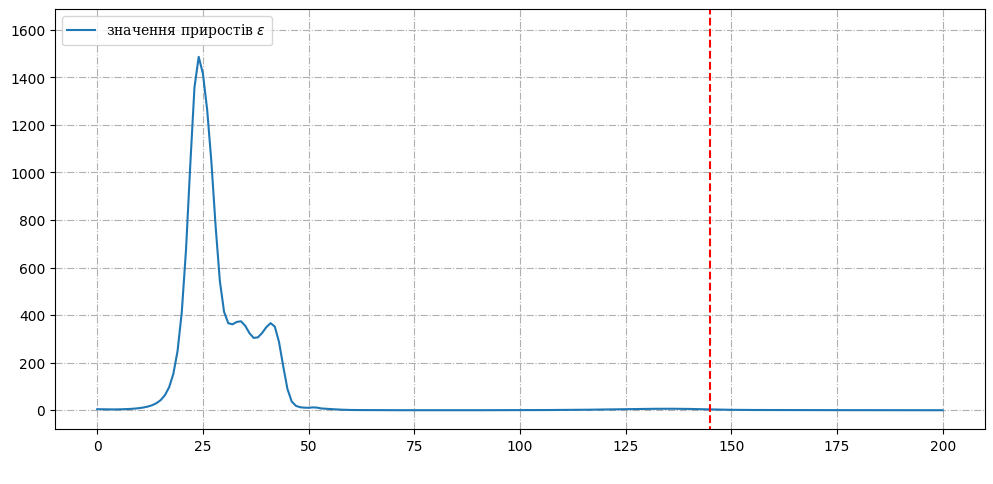
\includegraphics[width=1\linewidth]{4D_epsilon.png}}
    \end{minipage}
    \begin{minipage}[H]{1\linewidth}
        \center{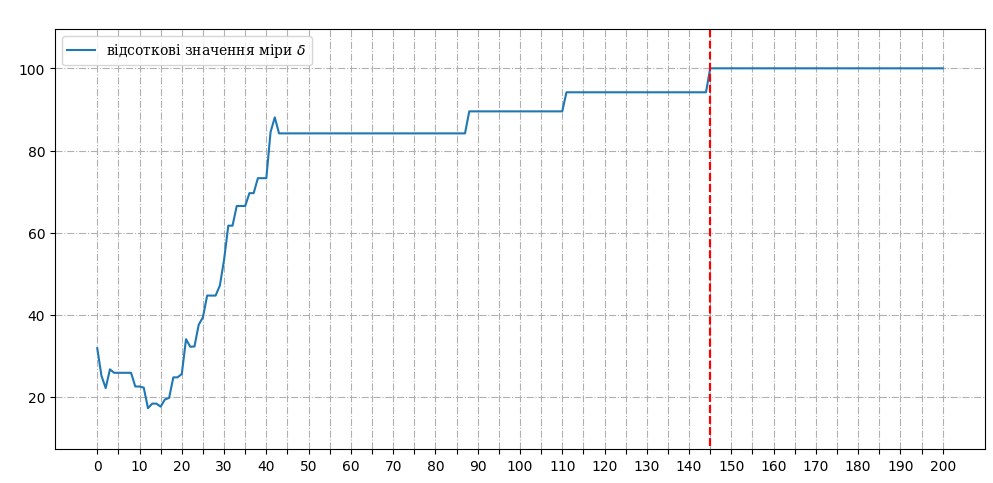
\includegraphics[width=1\linewidth]{4D_delta.png}}
    \end{minipage}
    \vspace{-0.4cm}
    \caption{Значення приростів $\varepsilon$ та міри $\delta$ від ітерації до ітерації}
    \label{figure: IV epsilon & delta}
\end{figure}

Порівнявши швидкості збіжності на Рис. \ref{figure: III epsilon & delta} та Рис. \ref{figure: IV epsilon & delta}, можна зауважити, що хоч алгоритм поділу на три та чотири кластери збігся за майже аналогічну кількість ітерацій ($n=143$ проти $n=145$), характер збіжності алгоритмів зовсім різний, що наочно проглядається при порівнянні графіків приростів $\varepsilon$ та значень міри $\delta$.

З графіку приростів $\varepsilon$ (Рис. \ref{figure: IV epsilon (0,15)-(200,600)}) робимо висновок, що серед наявних мінімумів у допустимих точках $B,C,D,E$ та $F$, найменшим є значення приросту у точці $F:$

\begin{figure}[H]
    \center{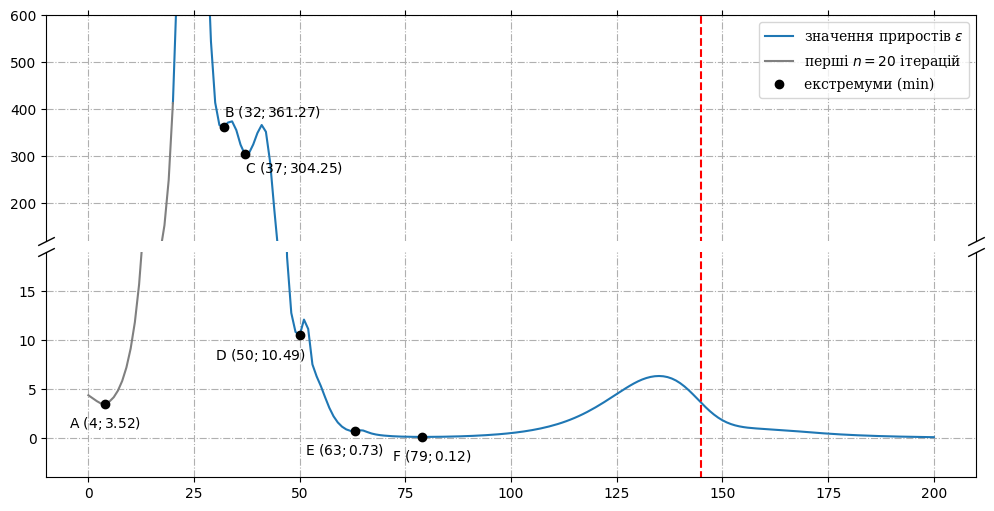
\includegraphics[width=1\linewidth]{4D_epsilon_zoom.png}}
    \vspace{-0.7cm}
    \caption{Значення $\varepsilon$ на проміжках $(0,15)$ та $(200,600)$}
    \label{figure: IV epsilon (0,15)-(200,600)}
\end{figure}

Отже, виконавши перші декiлька десяткiв iтерацiй, алгоримт Баума-Вешла можна зупиняти при першому спостереженні приросту $\varepsilon^*<0.12$.

\subsubsection{Результати та прикінцеві зауваження}

Використовуючи алгоритм навчання Баума-Велша, було отримано такі результати задачі кластеризації на дві, три та чотири кластери:

\vspace{0.4cm}
\begin{table}[H]
    \begin{center}
        \begin{tabular}{||c|c|c|l|l||}
            \hline
            Категорії & 
            \parbox{2.29cm}{\centering Модель $\lambda^0$} & 
            \parbox{3.8cm}{\centering Результати кластеризації} & 
            \parbox{2.4cm}{\centering Ітерація збіжності} & 
            \parbox{2.8cm}{\vspace{0.3cm}\centering Критерій зупинки алгоритму \vspace{0.2cm}} \\
            \hline
            I, II 
                & стp. \pageref{section: II classes} 
                & розподіл \ref{formula: II classes}
                & \quad $n=46$
                & \ $\varepsilon^*<42.85$ \\
            I, II, III 
                & стp. \pageref{section: III classes} 
                & розподіл \ref{formula: III classes} 
                & \quad $n=143$
                & \ $\varepsilon^*<12$ \\
            I, II, III, IV 
                & стp. \pageref{section: IV classes} 
                & розподіл \ref{formula: IV classes} 
                & \quad $n=145$
                & \ $\varepsilon^*<0.12$ \\
            \hline
        \end{tabular}
    \end{center}
    \caption{Результати задачі кластеризації}
    \label{table: results}
\end{table}

Зауважимо, що наведені результати справедливі лише для вказаних моделей $\lambda^0$, зокрема для фіксованих векторів $\mu^0$, матриць $A^0$ та $B^0$. Більш того, оскільки рівномірні матриці $B^0$ формуються випадковим чином (згідно правил, наведених на стр.~\pageref{section: II classes}), в інших дослідників не вийде відтворити графіки збіжності алгоритмів (Рис. \ref{figure: II delta}, \ref{figure: II epsilon}, \ref{figure: III epsilon & delta} та \ref{figure: IV epsilon & delta}) з точністю до аналогічної кількості екстремумів чи  відповідних значень $\varepsilon^*$.

Проте, виконавши значну кількість рестартів для $B^0$, спостереження стосовно загальних тенденцій, притаманних розглянутим алгоритмам кластеризації, можуть бути сформульовані таким чином:

\vspace{0.4cm}
\begin{table}[H]
    \begin{center}
        \begin{tabular}{||c|c|c|c|c||}
            \hline
            Категорії &  
            \parbox{4cm}{\centering Перші $n$ обов'язкових ітерацій} & 
            \parbox{4cm}{\centering Ітерація збіжності} & 
            \parbox{2.8cm}{\vspace{0.3cm}\centering Критерій зупинки алгоритму \vspace{0.2cm}} \\
            \hline
            I, II 
                & \multirow{3}{*}{$n\sim 50$} 
                & $n\sim 100$
                & \multirow{3}{*}{$\varepsilon^*<0.4$} \\
            I, II, III 
                & 
                & $n\sim 200$
                & \\
            I, II, III, IV 
                & 
                & $n\sim 200$
                & \\
            \hline
        \end{tabular}
    \end{center}
    \caption{Узагальнені спостереження}
    \label{table: main results}
\end{table}

Токаж варто зазначити, чому на жодній з візуалізацій цього роздлілу не відслідковується збіжність алгоритму впритул до еталонних $n=400$ ітерацій: після $n=80$ ітерацій у випадку двох категорій чи після $n=200$ ітерацій у випадках трьох та чотирьох категорій, прирости $\varepsilon$ або стрімко спадають, або якщо і мають певні точки екструмумів, то ці значення нехтовно малі.

Наостанок, наведемо у таблиці нижче порівняльну характеристику часу виконання алгоритмів кластеризації за, наприклад, $n=100$ ітерацій:

\vspace{0.4cm}
\begin{table}[H]
    \begin{center}
        \begin{tabular}{||c|c|c||}
            \hline
            Кількість ітерацій & Кількість категорій & \parbox{4cm}{\vspace{0.2cm}\centering Час виконання  алгоритму \vspace{0.2cm}} \\
            \hline
            \multirow{3}{*}{$n=100$} & I, II & $3{,}28$ хв \\
            & I, II, III & $5{,}51$ хв \\
            & I, II, III, IV & $8{,}36$ хв \\
            \hline
        \end{tabular}
    \end{center}
    \caption{Порівняльна таблиця часу виконання алгоритму}
\end{table}

\newpage
\subsection{Приклад: дешифрування тексту}
\label{section: text decoding by Baum-Welch}

Іншим прикладом використання алгоритму Баума-Велша в задачах кластеризації може слугувати декодування зашифрованого (наприклад, шифром Цезаря) тексту, кількість символів в якому $T\approx 100\ 000$. Суть завдання полягатиме в аналізі результатів алгоритму навчання деякої початкової моделі, сформованої згідно припущень про закодований текст, та виявленні для кожної літери шифру відповідної літери оригінального тексту.

Отже, з формальної точки зору задача звучатиме так: пара $\left\{(X_t,Y_t)\right\}_{t=\overline{0,T}}$ -- прихована марковська модель. Послідовність букв оригінального тексту $\left\{ X_t \right\}_{t=\overline{0,T}}$ задана на множині літер $E=\left\{e_1,e_2, \ldots, e_M\right\}$, а послідовність спостережуваних символів шифру $\left\{ Y_t \right\}_{t=\overline{0,T}}$ задана на алфавіті $F=\left\{f_1,f_2, \ldots, f_M\right\}$ деякої мови. Тоді задача кластеризації полягатиме у встановленні кожному символу з $F$ відповідного символу з множини $E$.

Оскільки вектор спостережуваних символів має значну довжину, то, знову ж таки, для алгоритму Баума-Велша справедливі модифікації, наведені у підрозділах <<Шкалювання алгоритмів прямого та зворотного ходу>> та <<Критерій зупинки алгоритму>>.

Для задачі дешифрування взято IV-X глави роману <<Місто>> автора Валер'яна Підмогильного. Тож в якості передпрограмного етапу підготуємо такі дві версії обраного тексту: 

\begin{align*}
    &\text{<<оригінальний>> текст} && \parbox{10.5cm}{очищена версія початкового тексту: залишені лише літери українського алфавіту (відповідно, без знаків пробілу та построфа) \vspace{0.2cm}} \\
    &\text{<<зашифрований>>  текст} && \parbox{10cm}{зашифрована версія <<оригінального>> тексту} \\
\end{align*}

Наприклад, розгялянемо уривок:

\vspace{0.4cm}
\begin{mdframed}[style=text box]
    \hspace{\tabsize}\textsl{
    Проблема грошей набувала дедалі загрозливіших форм. Він був напередодні банкротства всього свого вбрання від кашкета до галош, що, послуживши йому півроку, починало виявляти ознаки страшного, хоч і природного занепаду, якого годі було вже приховати ретельним чищенням. Процес одягання, такий приємний йому колись, тепер у сущу муку обернувся, бо вранці наявніш, ніж будь-коли, показувалась руїна його білизни, крайнє зужиття черевиків та лихий блиск ліктів на піджаку, віщун майбутньої дірки.}
\end{mdframed}

\vspace{0.4cm}
<<Оригінальна>> версія цього уривку матиме вид:

\newpage
\begin{mdframed}[style=text box]
    \hspace{\tabsize}\textsl{
    проблемагрошейнабуваладедалізагрозливішихформвінбувнапередоднібанкр\linebreak
    отствавсьогосвоговбраннявідкашкетадогалошщопослужившийомупіврокупочин\linebreak
    аловиявлятиознакистрашногохочіприродногозанепадуякогогодібуловжеприхова\linebreak тиретельнимчищеннямпроцесодяганнятакийприємниййомуколисьтеперусущуму\linebreak 
    куобернувсябовранцінаявнішніжбудьколипоказувасьруїнайогобілизникрайнєзу\linebreak
    життячеревиківталихийблискліктівнапіджакувіщунмайбутньоїдірки}
\end{mdframed}

\vspace{0.4cm}
В той час як <<зашифрована>> шифром Цезаря:

\vspace{0.4cm}
\begin{mdframed}[style=text box]
    \hspace{\tabsize}\textsl{
    тусдоипгжусїимргдцегогзизговкгжусколевїлшчсупеврдцергтиуизсзрвдгрну\linebreak схфхегефясжсфесжседугррбевзнгїнихгзсжгосїьстсфоцйлеїлмспцтвеуснцтсґлрго\linebreak
    селбеобхлскргнлфхугїрсжсшсґвтулусзрсжскгритгзцбнсжсжсзвдцосейитулшсегх\linebreak 
    луихиоярлпґльиррбптусщифсзбжгррбхгнлмтуліпрлммспцнсолфяхитиуцфцьцп\linebreak
    цнцсдиурцефбдсеугрщвргбервїрвйдцзянсолтснгкцегогфяуцюргмсжсдволкрлнуг\linebreak
    мрікцйлххбґиуиелнвехголшлмдолфновнхвергтвзйгнцевьцрпгмдцхрясюзвунл}
\end{mdframed}

\vspace{0.4cm}
Для подальшого формування початкової моделі $\lambda^0$ необхідні обидва варіанти тестів: як оригінальний, так і зашифрований. Шифровка тексту у прикладі здійснювалася шифром Цезаря, тобто зсувом кожної букви алфавіту на три позиції вперед:

\vspace{0.4cm}
\begin{table}[H]
    \setlength{\tabcolsep}{3.3pt}
    \renewcommand{\arraystretch}{0.5}
    \begin{center}
        \begin{tabular}{ccccccccccccccccccccccccccccccccc}
            а&б&в&г&д&е&ж&з&и&й&к&л&м&н&о&п&р&с&т&у&ф&х&ц&ч&ш&щ&ґ&ї&ь&є&ю&я&і \\
\rule[0pt]{0.8pt}{4pt} & \rule[0pt]{0.8pt}{4pt} & \rule[0pt]{0.8pt}{4pt} & \rule[0pt]{0.8pt}{4pt} & 
\rule[0pt]{0.8pt}{4pt} & \rule[0pt]{0.8pt}{4pt} & \rule[0pt]{0.8pt}{4pt} & \rule[0pt]{0.8pt}{4pt} & 
\rule[0pt]{0.8pt}{4pt} & \rule[0pt]{0.8pt}{4pt} & \rule[0pt]{0.8pt}{4pt} & \rule[0pt]{0.8pt}{4pt} & 
\rule[0pt]{0.8pt}{4pt} & \rule[0pt]{0.8pt}{4pt} & \rule[0pt]{0.8pt}{4pt} & \rule[0pt]{0.8pt}{4pt} &
\rule[0pt]{0.8pt}{4pt} & \rule[0pt]{0.8pt}{4pt} & \rule[0pt]{0.8pt}{4pt} & \rule[0pt]{0.8pt}{4pt} &
\rule[0pt]{0.8pt}{4pt} & \rule[0pt]{0.8pt}{4pt} & \rule[0pt]{0.8pt}{4pt} & \rule[0pt]{0.8pt}{4pt} &
\rule[0pt]{0.8pt}{4pt} & \rule[0pt]{0.8pt}{4pt} & \rule[0pt]{0.8pt}{4pt} & \rule[0pt]{0.8pt}{4pt} &
\rule[0pt]{0.8pt}{4pt} & \rule[0pt]{0.8pt}{4pt} & \rule[0pt]{0.8pt}{4pt} & \rule[0pt]{0.8pt}{4pt} &
\rule[0pt]{0.8pt}{4pt} \\
            г&д&е&ж&з&и&й&к&л&м&н&о&п&р&с&т&у&ф&х&ц&ч&ш&щ&ґ&ї&ь&є&ю&я&і&а&б&в \\
        \end{tabular}
    \end{center}
    \caption{Шифрувальна таблиця}
    \label{table: true cipher}
\end{table}

Тож на кінець підготовчого етапу отримуємо оригінальний та зашифрований тексти ($T=112\; 216$ символів), задані на алфавіті $F$ довжиною $M=33$ елементи:
\begin{equation}
    F=\{\text{<<а>>},\text{<<б>>},\text{<<в>>},\ldots,\text{<<ь>>},\text{<<є>>},\text{<<ю>>},\text{<<я>>},\text{<<і>>}\}
    \label{formula: UKR chipher alphabet}
\end{equation}

Останнім кроком перед запуском самого алгоритму навчання задамо початкову модель $\lambda^0$ таким чином:
\begin{enumerate}
    \item[$A^0:$] На основі аналізу оригінального тексту визначимо компоненти $\widetilde{A}_{ij}$ як кiлькiсть спостережень впорядкованої пари букв $(i, j)$ у  заданому текстi. Наступним кроком для виконання умови стохастичності матриці, а також задля невід'ємності її елементів, додамо до кожного $\widetilde{A}_{ij}$ число 5, а потiм віднормуємо матрицю, подiливши кожен елемент на суму елементiв вiдповiдної стрiчки:
    \[ \forall i\in E: \quad A_{ij}^0=\frac{\widetilde{A}_{ij}}{\sum\limits_{j\in F}\widetilde{A}_{ij}} \]

    \item[$B^0:$] Аби якнайкраще відповідати характеристикам наданого тексту (чутливість алгоритму до початкових параметрів прослідковувалася й раніше), побудуємо $B^0$ на основі результатів кластеризації літер на голосні-приголосні, використовуючи методологію попередніх розділів. Наприклад, групи голосних та приголосних, сформованих в результаті аналізу оригінального тексту, позначимо як $C$ (consonants) та $V$ (vowels) відповідно. А результати аналізу зашифрованого тексту -- як $C^{\text{\scriptsize \#}}$ й $V^{\text{\scriptsize \#}}$.  Тоді $B^0$ формуватиметься так:
    \begin{equation*}
        \forall i\in E, \forall j\in F: \quad B_{ij}^0=
        \begin{cases}
            \sim\frac{1}{|C^{\text{\tiny \#}}|}, & i\in C, j\in C^{\text{\scriptsize \#}} \\
            \sim 0, & i\in C, j\in V^{\text{\scriptsize \#}} \\
            \sim\frac{1}{|V^{\text{\tiny \#}}|}, & i\in V, j\in V^{\text{\scriptsize \#}} \\
            \sim 0, & i\in V, j\in C^{\text{\scriptsize \#}}\\
        \end{cases}
    \end{equation*}

    \item[$\mu^0:$] Покладемо вектор початкового розподілу як інваріантний розподіл ланцюга Маркова, тобто як розв'язок такого рівняння:
    \[ \mu^0A=\mu^0, \]

    де $A$ -- сформована у першому пункті матриця перехідних імовірностей.
\end{enumerate}

Зважаючи на те, що початкова модель $\lambda^0$ формується, крім іншого, й на основі незашифрованого тексту, розв'язок задачі декодування є радше демонстративним, аніж дослідницьким. 

Нарешті, запустимо процес виконання алгоритму навчання для заданої моделі $\lambda^0=(\mu^0,A^0,B^0)$, враховуючи, що процес переоцінення слід виконувати лише для вектора $\mu$ та матриці $B$. Крім того, в якості ланцюжка спостережень слід взяти лише перші $1000$ символів зашифрованого тексту.

\subsubsection*{Результати}

Отримавши в результаті роботи $n=200$ ітерацій переоцінену матрицю $B^*$, віднесемо кожен символ $i$ з множини $F$ символу $j$ з множини $E$ таким чином: 
\[ \forall i\in F: j=arg\max\limits_{j\in E} B^*_{ij} \]

Утворена шифрувальна таблиця матиме вид:
\vspace{0.4cm}
\begin{table}[H]
    \setlength{\tabcolsep}{3.3pt}
    \renewcommand{\arraystretch}{0.5}
    \begin{center}
        \begin{tabular}{ccccccccccccccccccccccccccccccccc}
            а&б&в&г&д&е&ж&з&и&й&к&л&м&н&о&п&р&с&т&у&ф&х&ц&ч&ш&щ&ґ&ї&ь&є&ю&я&і \\
\rule[0pt]{0.8pt}{4pt} & \rule[0pt]{0.8pt}{4pt} & \rule[0pt]{0.8pt}{4pt} & \rule[0pt]{0.8pt}{4pt} & 
\rule[0pt]{0.8pt}{4pt} & \rule[0pt]{0.8pt}{4pt} & \rule[0pt]{0.8pt}{4pt} & \rule[0pt]{0.8pt}{4pt} & 
\rule[0pt]{0.8pt}{4pt} & \rule[0pt]{0.8pt}{4pt} & \rule[0pt]{0.8pt}{4pt} & \rule[0pt]{0.8pt}{4pt} & 
\rule[0pt]{0.8pt}{4pt} & \rule[0pt]{0.8pt}{4pt} & \rule[0pt]{0.8pt}{4pt} & \rule[0pt]{0.8pt}{4pt} &
\rule[0pt]{0.8pt}{4pt} & \rule[0pt]{0.8pt}{4pt} & \rule[0pt]{0.8pt}{4pt} & \rule[0pt]{0.8pt}{4pt} &
\rule[0pt]{0.8pt}{4pt} & \rule[0pt]{0.8pt}{4pt} & \rule[0pt]{0.8pt}{4pt} & \rule[0pt]{0.8pt}{4pt} &
\rule[0pt]{0.8pt}{4pt} & \rule[0pt]{0.8pt}{4pt} & \rule[0pt]{0.8pt}{4pt} & \rule[0pt]{0.8pt}{4pt} &
\rule[0pt]{0.8pt}{4pt} & \rule[0pt]{0.8pt}{4pt} & \rule[0pt]{0.8pt}{4pt} & \rule[0pt]{0.8pt}{4pt} &
\rule[0pt]{0.8pt}{4pt} \\
            г&д&е&ж&з&и&й&к&л&м&н&о&п&р&с&т&у&ф&х&ц&{\color{blue}к}&ш&щ&ґ&ї&{\color{blue}ш}&{\color{blue}к}&ю&я&{\color{blue}ї}&а&б&в \\
        \end{tabular}
    \end{center}
    \caption{Шифрувальна таблиця}
\end{table}

Порівнявши з Табл. \ref{table: true cipher} отримані відповідності, можна помітити, що чотири літери розшифровано неправильно (помилкові літери виділені синім кольором). Відтак відсоток правильно декодованих літер складає 88\%.

\newpage
Прослідкуємо за приростами логарифмів ймовірностей та за зростанням відсотку правильно вгаданих літер від ітерації до ітерації:

\begin{figure}[H]
    \center{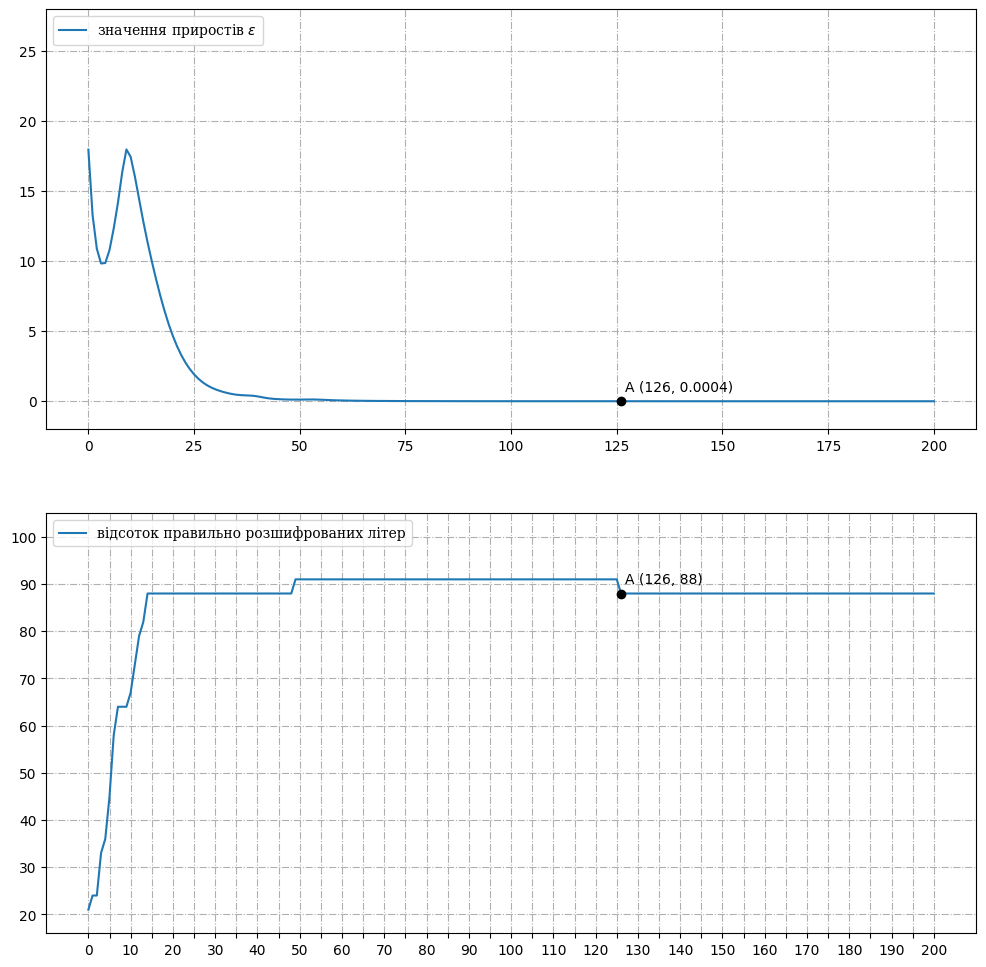
\includegraphics[width=1\linewidth]{Bvc_Minv.png}}
    \caption{Початкова модель $\lambda^0=(A^0,B^0_\text{голосні/приголосні},\mu^0_\text{стаціонарний})$}
    \label{figure: Bvc + Minv}
\end{figure}

Назагал, модель демонструє незначні стрибки зростання та подальше стрімке спадання значень $\varepsilon$. Точкою $A$ позначена координата ітерації $n=126$, за якої відсоток правильно розшифрованих літер вперше сягає 88\% й надалі не змінюється (на сотні ітерацій вперед).

Окремої уваги заслуговують й інші конфігурації початкової моделі $\lambda^0$. Наприклад, схожий характер збіжності прослідковується при аналогічному формуванні матриці $B^0$, проте при заданні початкового розподілу $\mu^0$ рівномірним (Рис. \ref{figure: Bvc + Muni}).

\begin{figure}[H]
    \center{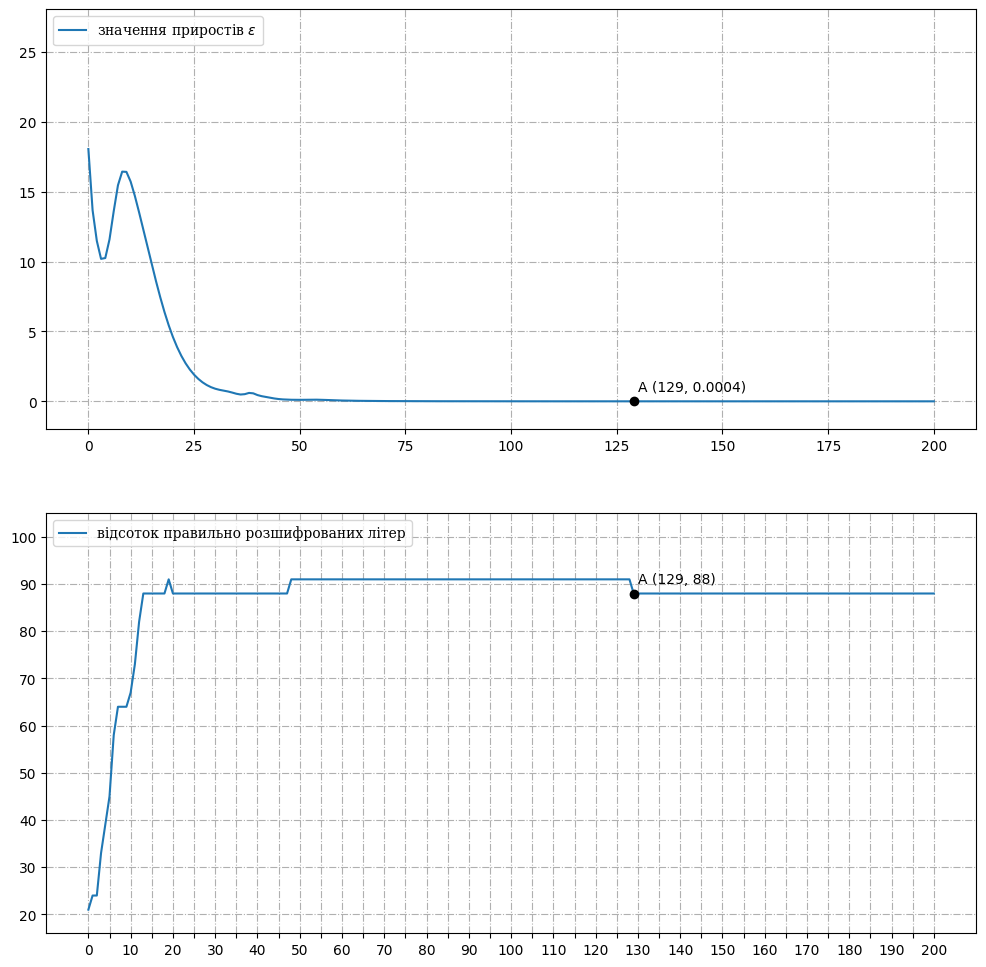
\includegraphics[width=1\linewidth]{Bvc_Muni.png}}
    \caption{Початкова модель $\lambda^0=(A^0,B^0_\text{голосні/приголосні},\mu^0_\text{рівномірний})$}
    \label{figure: Bvc + Muni}
\end{figure}

Бачимо, що швидкість збіжності хоч і менша, проте не набагато: вже за $n=129$ ітерацій відсоток досягає аналогічних 88\%. 

Натомість, при спробі задати початкові параметри як матриці $B^0$, так і вектора $\mu^0$ рівномірним чином (Рис. \ref{figure: Buni + Muni}), збіжність триває значно довше, включно до ітерації $n=167$. Водночас, прирости $\varepsilon$ зростають протягом перших ітерацій більш інтенсивно, що можна пояснити відсутністю в матриці $B$ певної <<підказки>>, як це було раніше. 

\begin{figure}[H]
    \center{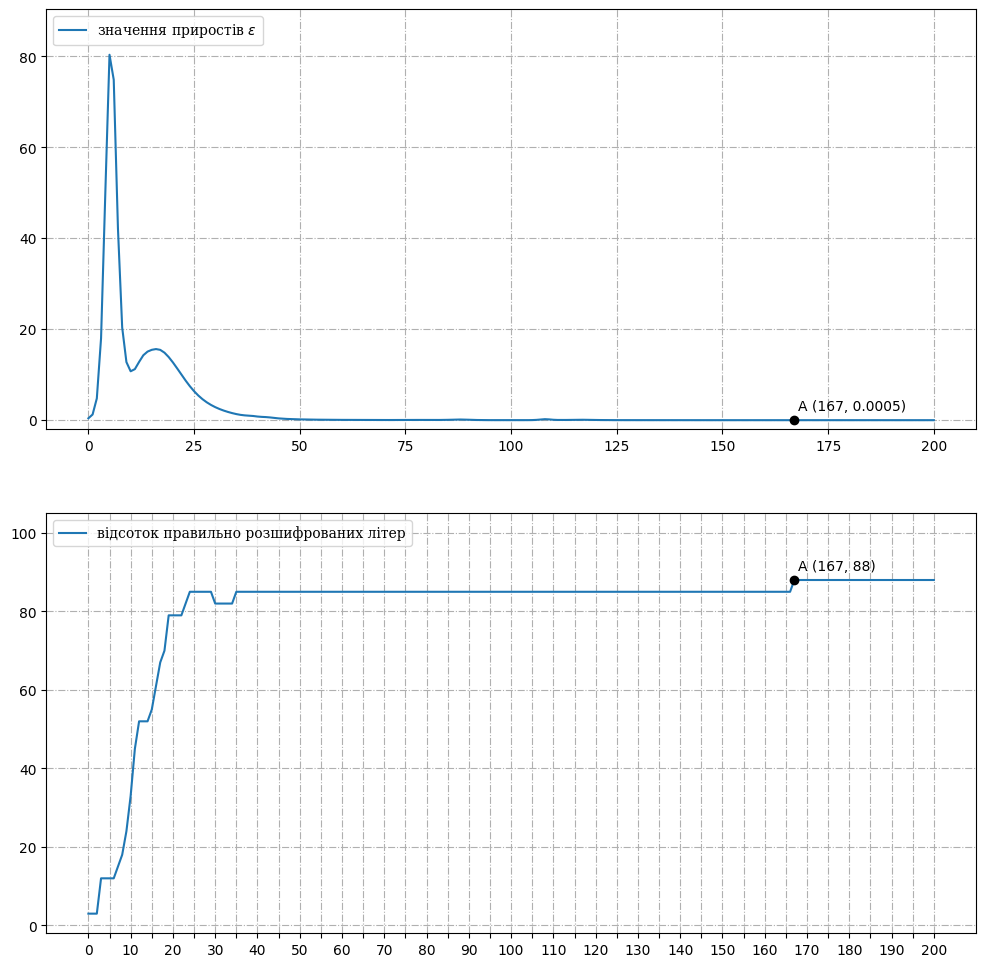
\includegraphics[width=1\linewidth]{Buni_Muni.png}}
    \caption{Початкова модель $\lambda^0=(A^0,B^0_\text{рівномірна},\mu^0_\text{рівномірний})$}
    \label{figure: Buni + Muni}
\end{figure}

Отже, хоч збіжність триває і довше, рівномірні початкові параметри (за винятком матриці $A^0$, яка в усіх випадках має формуватися як частотний аналіз оригінального тексту) також демонструють хороші результати. Чого зовсім не скажеш про останню з можливих комбінацій, яка буде розглянута нижче.

Тож четвертим варіантом набору початкових параметрів є комбінація рівномірної матриці $B^0$ та стаціонарного розподілу $\mu^0$ (Рис. \ref{figure: Buni + Minv}). Прикро, проте у такому випадку модель зовсім не покращується, тобто відсоток правильно вгаданих літер сягає виключно нульового значення.

\begin{figure}[H]
    \center{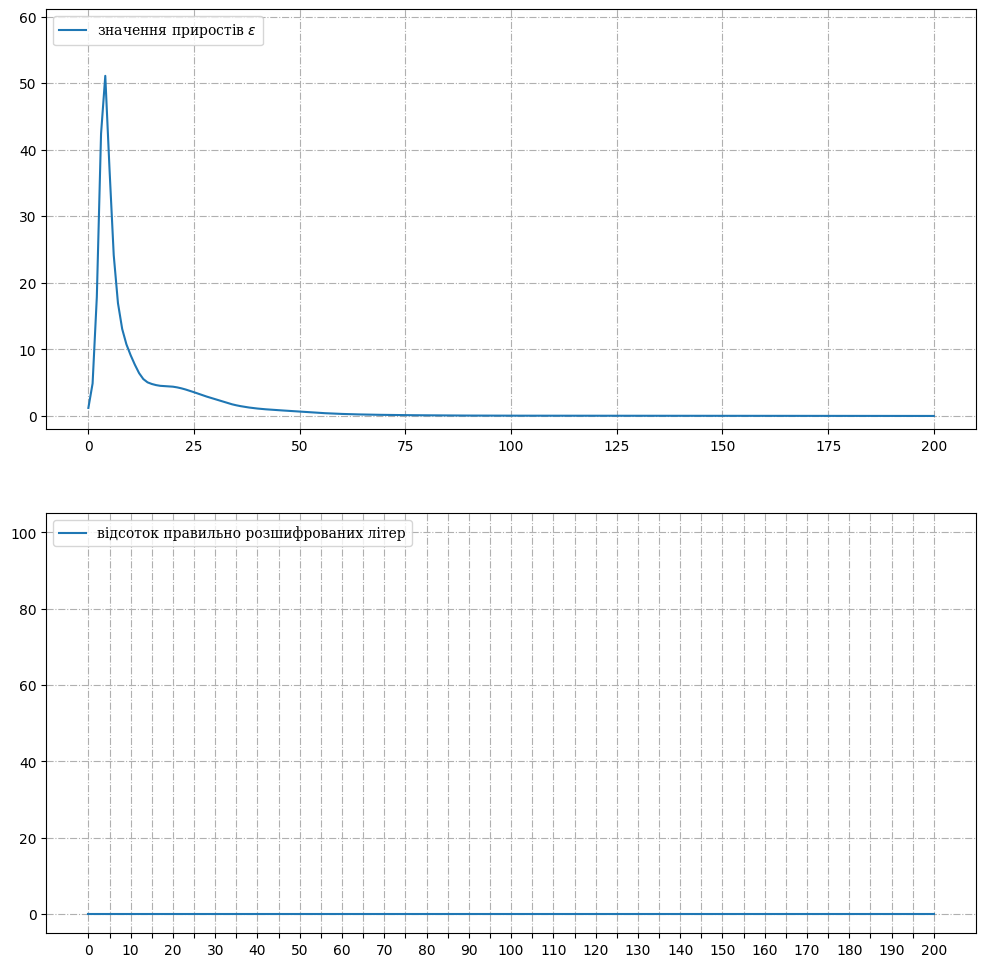
\includegraphics[width=1\linewidth]{Buni_Minv.png}}
    \caption{Початкова модель $\lambda^0=(A^0,B^0_\text{рівномірна},\mu^0_\text{стаціонарний})$}
    \label{figure: Buni + Minv}
\end{figure}